\documentclass[tikz,border=5pt,png]{standalone}
\usepackage{tikz}
\usetikzlibrary{shapes.geometric, positioning, arrows.meta}

\definecolor{Green}{HTML}{8ac478}
\definecolor{Yellow}{HTML}{f5ee6c}
\definecolor{Red}{HTML}{c95349}

\begin{document}
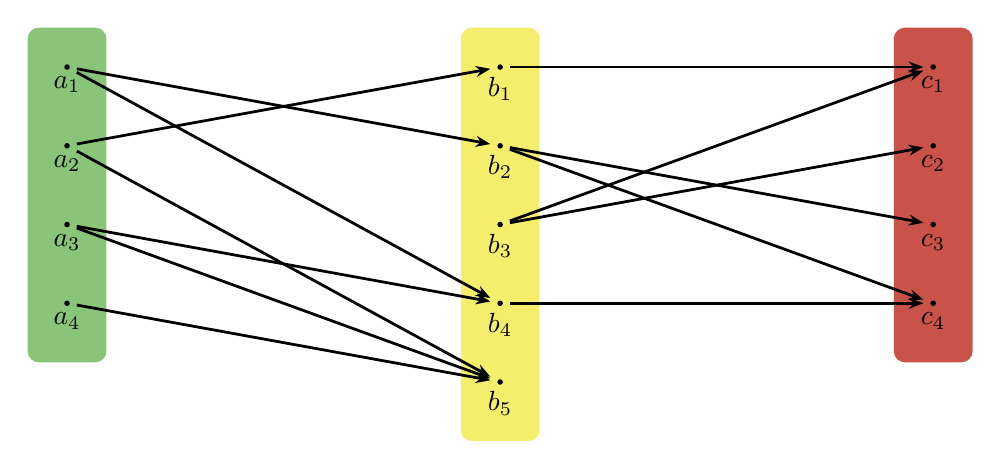
\begin{tikzpicture}[>={Stealth[scale=0.7]}]

\fill[Green,rounded corners] (-0.5, 0.5) rectangle (0.5, -3.75);

\node (a1) at (0,0) {};
\node (a2) at (0,-1) {};
\node (a3) at (0,-2) {};
\node (a4) at (0,-3) {};

\node (b1) at (5.5,0) {};
\node (b2) at (5.5,-1) {};
\node (b3) at (5.5,-2) {};
\node (b4) at (5.5,-3) {};
\node (b5) at (5.5,-4) {};

\node (c1) at (11,0) {};
\node (c2) at (11,-1) {};
\node (c3) at (11,-2) {};
\node (c4) at (11,-3) {};

\fill (a1) circle [radius=1pt] node[below]  {$a_1$};
\fill (a2) circle [radius=1pt] node[below] {$a_2$};
\fill (a3) circle [radius=1pt] node[below] {$a_3$};
\fill (a4) circle [radius=1pt] node[below] {$a_4$};

\fill[Yellow,rounded corners] (5, 0.5) rectangle (6, -4.75);
\fill[Red,rounded corners] (10.5, 0.5) rectangle (11.5, -3.75);

\fill (b1) circle [radius=1pt] node[below] {$b_1$};
\fill (b2) circle [radius=1pt] node[below] {$b_2$};
\fill (b3) circle [radius=1pt] node[below] {$b_3$};
\fill (b4) circle [radius=1pt] node[below] {$b_4$};
\fill (b5) circle [radius=1pt] node[below] {$b_5$};

\draw[->,line width=1pt] (a1) -- (b2);
\draw[->,line width=1pt] (a1) -- (b4);
\draw[->,line width=1pt] (a2) -- (b1);
\draw[->,line width=1pt] (a2) -- (b5);
\draw[->,line width=1pt] (a3) -- (b4);
\draw[->,line width=1pt] (a3) -- (b5);
\draw[->,line width=1pt] (a4) -- (b5);

\fill (c1) circle [radius=1pt] node[below] {$c_1$};
\fill (c2) circle [radius=1pt] node[below] {$c_2$};
\fill (c3) circle [radius=1pt] node[below] {$c_3$};
\fill (c4) circle [radius=1pt] node[below] {$c_4$};

\draw[->,line width=1pt] (b1) -- (c1);
\draw[->,line width=1pt] (b2) -- (c3);
\draw[->,line width=1pt] (b2) -- (c4);
\draw[->,line width=1pt] (b3) -- (c1);
\draw[->,line width=1pt] (b3) -- (c2);
\draw[->,line width=1pt] (b4) -- (c4);

\end{tikzpicture}
\end{document}

